% !TeX spellcheck = en_GB
\section{Measurement site - Haukeliseter}
\label{sec:site}
%%% images measurement site %%%%%%%%%%%%%%%%%%%%%%%%%%%%%%%%%%%%%
% !TeX spellcheck = en_GB
\begin{figure}[t]
	\centering
    \begin{subfigure}[b]{0.49\textwidth}
    	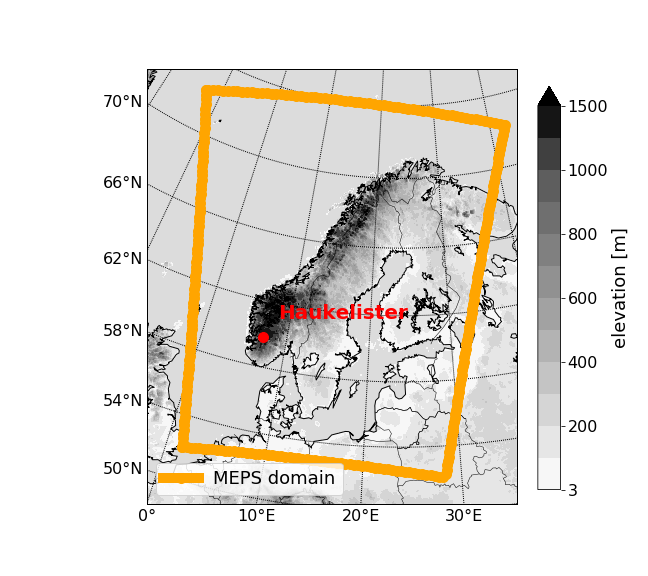
\includegraphics[trim={2.75cm 1.8cm 4.4cm 2.3cm},clip,
        width=\textwidth]{./fig_Norway/Norway_MEPS}
        \caption{}\label{fig:site:Norway}
    \end{subfigure}
 %%%%% zoomed in map
    \begin{subfigure}[b]{0.49\textwidth}
    	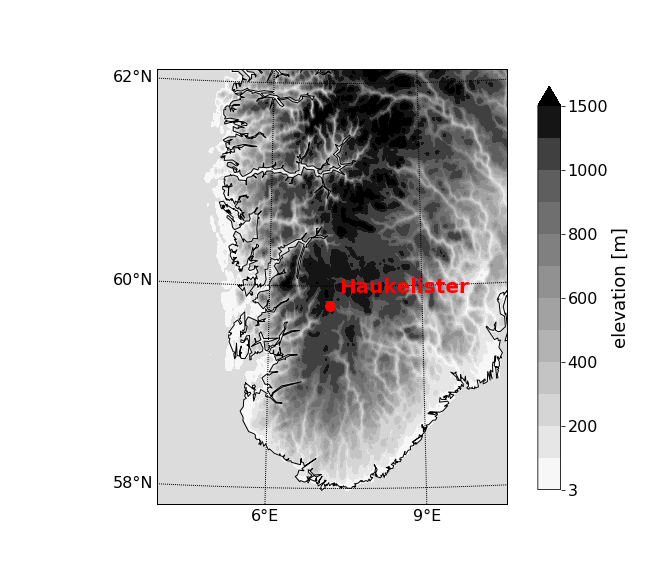
\includegraphics[trim={2.75cm 1.8cm .65cm 2.3cm},clip,
        width=\textwidth]{./fig_Norway/South_Norway}
    	\caption{}\label{fig:site:Nzoom}
    \end{subfigure}
   	\caption{Elevation map of Northern Europe and South Norway, \subref{fig:site:Norway}, \subref{fig:site:Nzoom} respectively. Red dot indicates the location Haukeliseter and the orange square in \subref{fig:site:Norway} indicates the model domain of MEPS. Elevation according to the shading.} \label{fig:site}
\end{figure}
%%%%%%%%%%%%%%%%%%%%%%%%%%%%%%%%%%%%%%%%%%%%%%%%%%%%%%%%%%%%%%%%%%%%%%%%%%
Haukeliseter, shown in \Cref{fig:site} is a mountain plateau \SI{991}{\m} above sea level, located in the Norwegian county 'Telemark' (\ang{59.8}\,N, \ang{7.2}\,E). The station measures precipitation, temperature, snow depth and wind. It has served as a measurement site for snow accumulation since the winter of 2010/2011 \citep{wolff_new_2010, wolff_measurements_2013, wolff_derivation_2015}. 
\\
In a study by \cite{wolff_derivation_2015} the wind-induced under-catch of solid precipitation is determined. Dependent on the kind of precipitation the wind plays different roles in the amount of accumulation. For temperatures below \SI{-2}{\celsius} the wind speed influences the falling snow. Where less precipitation can be observed at higher wind speeds or more precipitation can be measured if too much is blown into the gauge. The catch ratio between the standard Geonor precipitation gauge and the DF-Geonor shows, that only \SI{80}{\percent} of solid precipitation are observed at wind speeds of \SI{2}{\mPs} and only \SI{40}{\percent} at \SI{5}{\mPs}, \cite[Figure 5 in][]{wolff_derivation_2015}. The double fence gauge is more accurate than the single fence and is used as the reference gauge.
%\textcolor{red}{Steve: Should make some reference here to the vertical profile of observations needed to evaluate MEPS.  Me: What exactly does he mean?}. 
Nevertheless, this shows the need of a combination of ground based observations together with an optimal estimation retrieval to verify the accuracy of MEPS. \cite{wolff_derivation_2015} introduced an adjustment function for the Geonor double fence, so that different precipitation under certain wind speeds are presented correctly and can be used as confidential data. 